\documentclass[
        a4paper,
        10pt,
        parskip = full,    % Layout with zero \parident and non-zero \parskip
    ]{scrartcl}
% \usepackage[utf8]{inputenc}

\usepackage[top=2cm, bottom=2.5cm, left=2.5cm, right=2.5cm]{geometry}
\usepackage[
        colorlinks = true,    % Disable drawing boxes around links.
        linkcolor = black,    % Sets the color of links to black.
    ]{hyperref}
\usepackage{amsmath}
\usepackage{graphicx}
\usepackage{subfig}
\usepackage{float}

\begin{document}

\textbf{\large{Laboratory - Deep Learning Lab, WS 2018/2019 - Exercise 3}}

\textbf{\large{Submitted by: Amadeus Hovekamp,\\
mail@amadeus-hovekamp.de,\\
Matr. no: 4603934}}

The repository with the source code can be found under the following link:\\
\href{https://github.com/Schokokugel/RoboticsLab}
     {https://github.com/Schokokugel/RoboticsLab}

\section{Getting Set Up}

The set up of OpenAI Gym was fast and easy.

\section{Behavioral Cloning}
\subsection{Getting familiar and collection expert driving data}
At first it was strange that there is little to no friction slowing down the car
while driving. Hans N\"ubel and I observed different running speeds on different
machines making it really hard to collect good expert data on the faster computer.
For that reason I tried collecting expert data by adding a short pause between
every frame. Due to data loading time before training I collected four expert
data sets containing 5000, 10000, 20000 and 35000 data points. The histograms of actions
used are shown in figures \ref{dist_5000},  \ref{dist_10000}, \ref{dist_20000} and \ref{dist_35000}. As you can see the Action IDs go up to 8 as we added 4 additional IDs for the cases of two keys pressed at the same time. We added those IDs as we read that the $action\_to\_ID$ method is unable to handly multiple keys pressed at the same time and because we actually used two keys at the same time while driving manually.

There is a difference in the number of occurences of those added actions between the smalles dataset and the other sets. The reason for this is the necessity of having a big enough number of those samples to sample uniformly over all action IDs in a later step. The very small number of occurences in the expert data containing 10000 samples is due to the fact that I eventually stopped training the agent using those mixed action IDs. More choices makes it even harder for the agent to learn from the little data we can provide anyway.

\begin{figure}[H]
  \begin{center}
    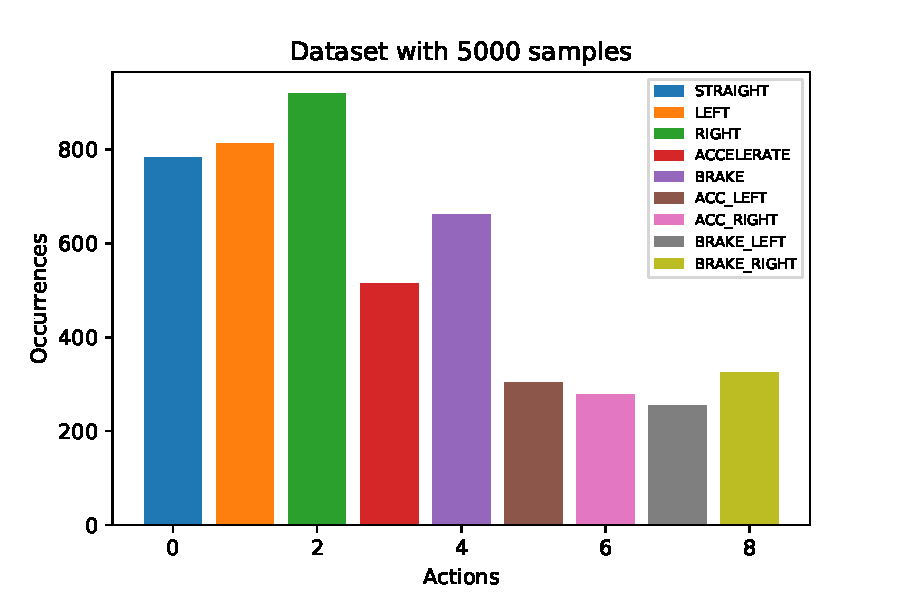
\includegraphics{../images/action_distribution_5000.pdf}
    \caption{Distributions of Action IDs in the expert data}
    \label{dist_5000}
  \end{center}
\end{figure}

\begin{figure}[H]
  \begin{center}
    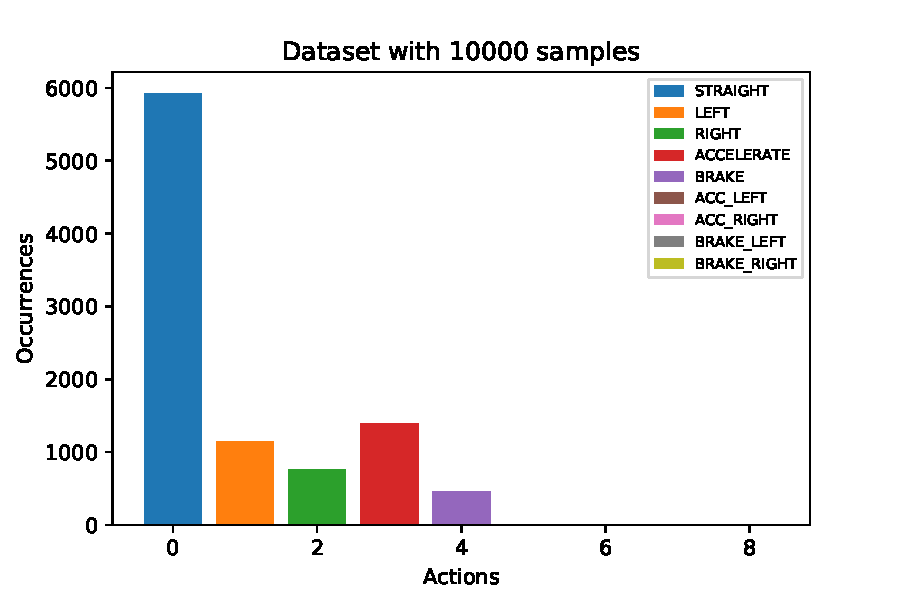
\includegraphics{../images/action_distribution_10000.pdf}
    \caption{Distributions of Action IDs in the expert data}
    \label{dist_10000}
  \end{center}
\end{figure}

\begin{figure}[H]
  \begin{center}
    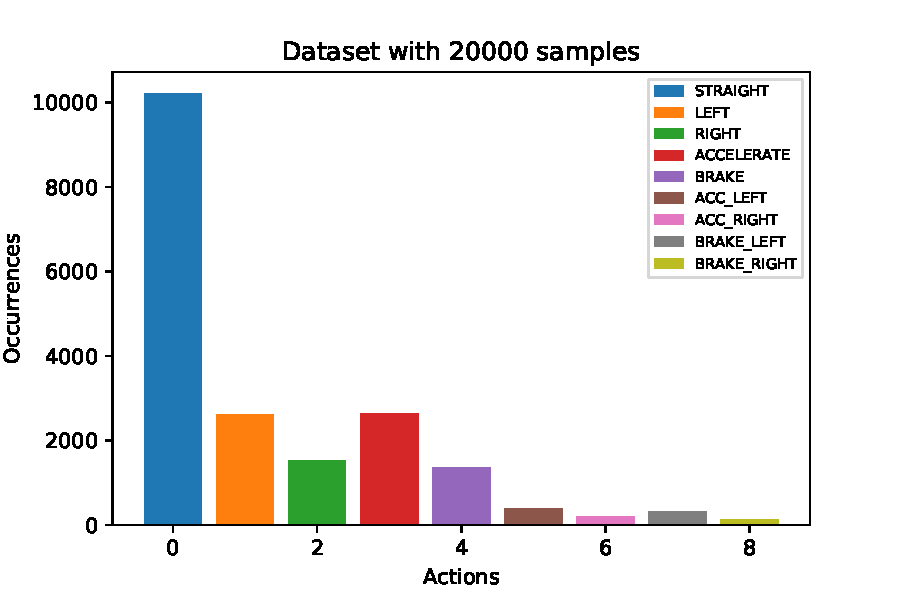
\includegraphics{../images/action_distribution_20000.pdf}
    \caption{Distributions of Action IDs in the expert data}
    \label{dist_20000}
  \end{center}
\end{figure}

\begin{figure}[H]
  \begin{center}
    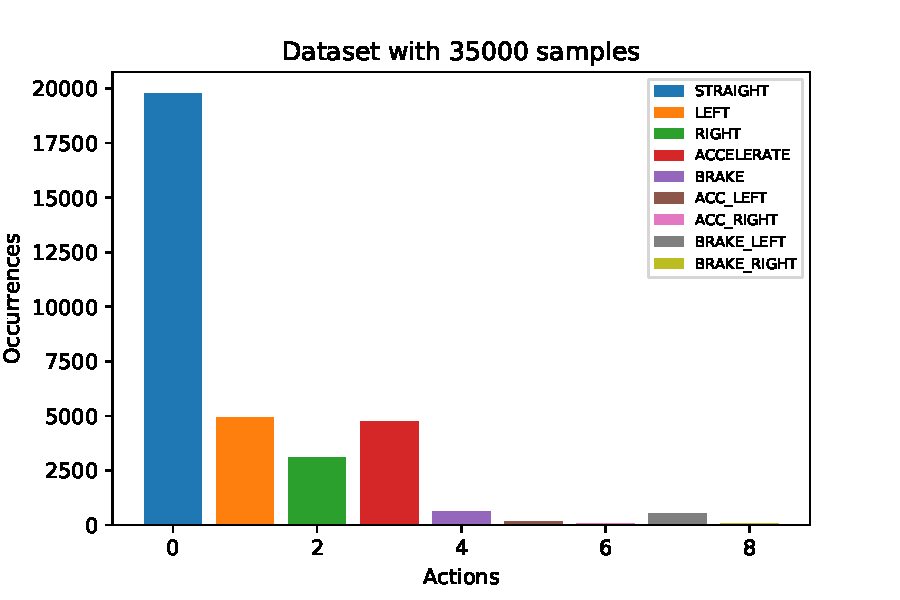
\includegraphics{../images/action_distribution_35000.pdf}
    \caption{Distributions of Action IDs in the expert data}
    \label{dist_10000}
  \end{center}
\end{figure}


\subsection{Creating and training a behavioral cloning agent}
Training a behavioral cloning agent took some time, as I solved exercise 2 using automated training, which ran a specified number of epochs with one command. To track the learning progress with TensorBoard, I had to run the training batch by batch in a loop.

\subsection{The first network}
We chose to run the network from the last exercise first.
It consists of the input layer, two convolutional layers, each followed by a max pooling layer, followed by a fully connected layer and the output layer. The both convolutional layers have 16 filters of size 3 by 3.

% TODO: Add train and valid, loss, accuracy and error plot
\begin{figure}[H]
  \begin{center}
    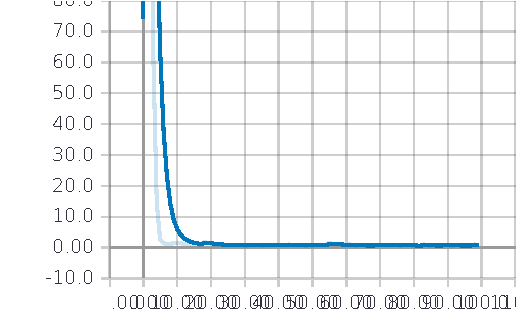
\includegraphics[width=10cm]{../images/loss.pdf}
    \caption{Loss of the improved network during training}
    \label{Learning measurements}
  \end{center}
\end{figure}

\begin{figure}[H]
  \begin{center}
    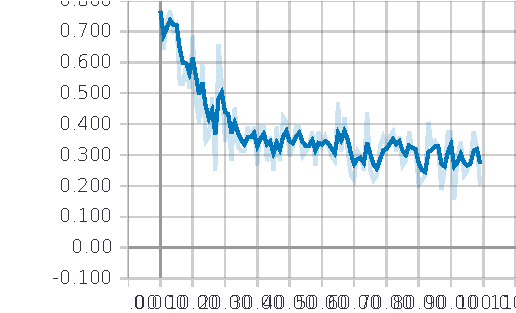
\includegraphics[width=10cm]{../images/train_error.pdf}
    \caption{Error of the first network during training}
    \label{Learning measurements}
  \end{center}
\end{figure}

\begin{figure}[H]
  \begin{center}
    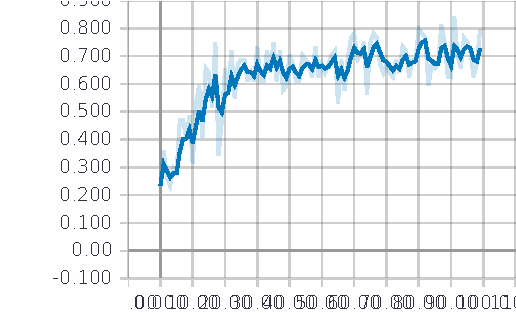
\includegraphics[width=10cm]{../images/train_accuracy.pdf}
    \caption{Training accuracy of the first network during training}
    \label{Learning measurements}
  \end{center}
\end{figure}

\begin{figure}[H]
  \begin{center}
    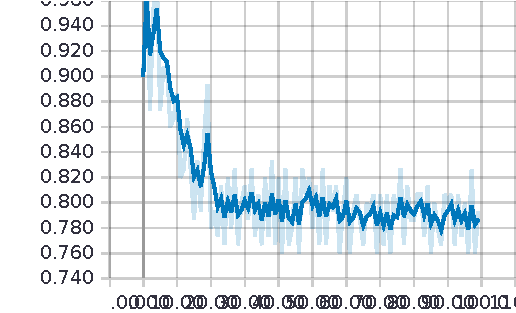
\includegraphics[width=10cm]{../images/valid_error.pdf}
    \caption{Validation error of the first network during training}
    \label{Learning measurements}
  \end{center}
\end{figure}

\begin{figure}[H]
  \begin{center}
    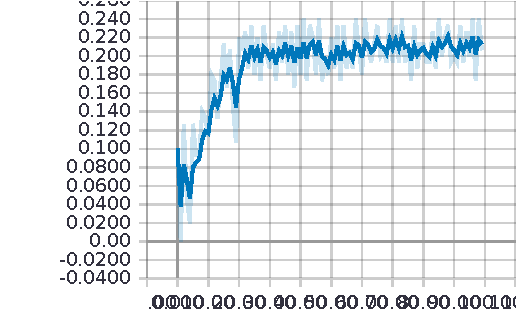
\includegraphics[width=10cm]{../images/valid_accuracy.pdf}
    \caption{Validation accuracy of the first network during training}
    \label{Learning measurements}
  \end{center}
\end{figure}

As one can see from the images showing the learning progress, this network was
not able to learn the steering patterns very well, having more than 30 \%
training error and almost 80 \% validation error. When testing this model
using the test_agent script, it performes really badly. Most of the time it
just does not accelerate at all at the start and therefore will not do until the
end of the episode. Sometimes it will just accelerate and drive straight.
This behavior of only chosing one action in every scenario was observed time and
time again.

\subsection{Balancing the training data}
As one can see in the figures displaying the action distributions, most of the
time the best possible action according to the expert data is to go STRAIGHT.
This unbalanced data may cause the agent to always choose this action and minimize
its loss this way. We therefore balanced the data by first uniformly choosing one
action ID and then adding a sample where the expert driver chose this action to
the minibatch.

This did not improve our results, especially because we added the additional
action ID, which rarely occured when not intentionally added by driving in a
special ways. So I decided to uniformly sample only the most commen steering commands.

\subsection{An improved network}
Dozens of trys to improve the network's performance by changing its architecture failed. I tried adding a second fully connected layer between the existing fully connected layer and the output layer, increasing the number of filters in the convolutional layers and several other things. But then we found a network which at least occasionaly performed substantially better that our first network.
We increased the kernel size in both convolution layers to 7.
And this actually helped a lot. Now the agent way able to indentify the street,
at least some times following it.
One interesting note is, that the agent acutally recognized the numbers in the
bottom left, always acceleration when a certain digit was visible.

\begin{figure}[H]
  \begin{center}
    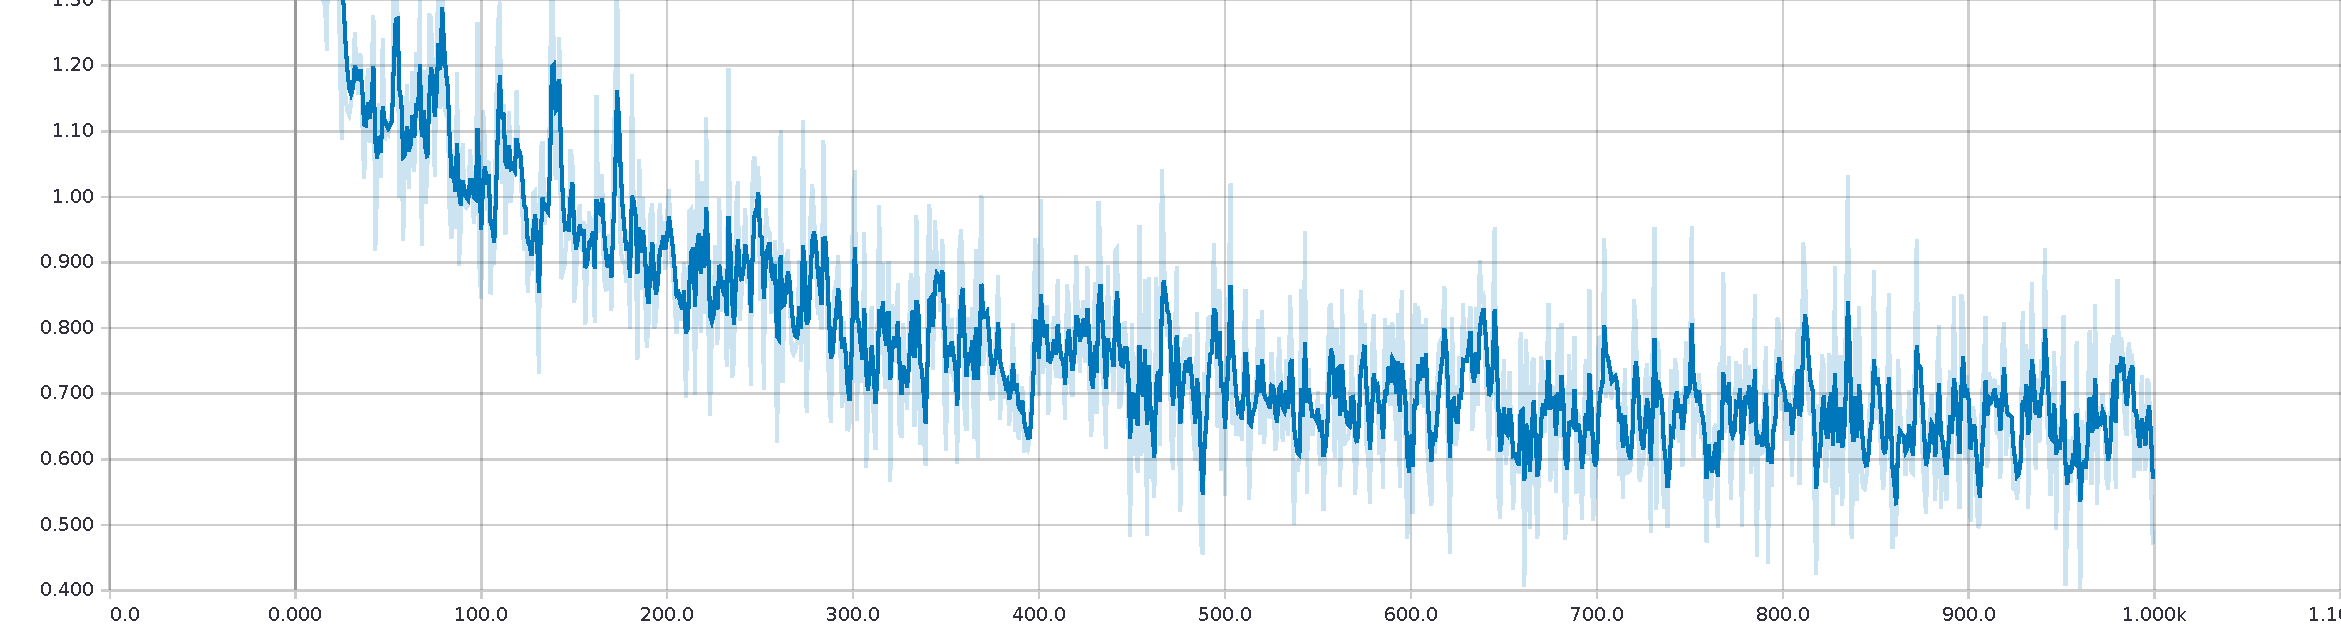
\includegraphics[width=16cm]{../images/improved_loss.pdf}
    \caption{Loss of the improved network during training}
    \label{Learning measurements}
  \end{center}
\end{figure}

\begin{figure}[H]
  \begin{center}
    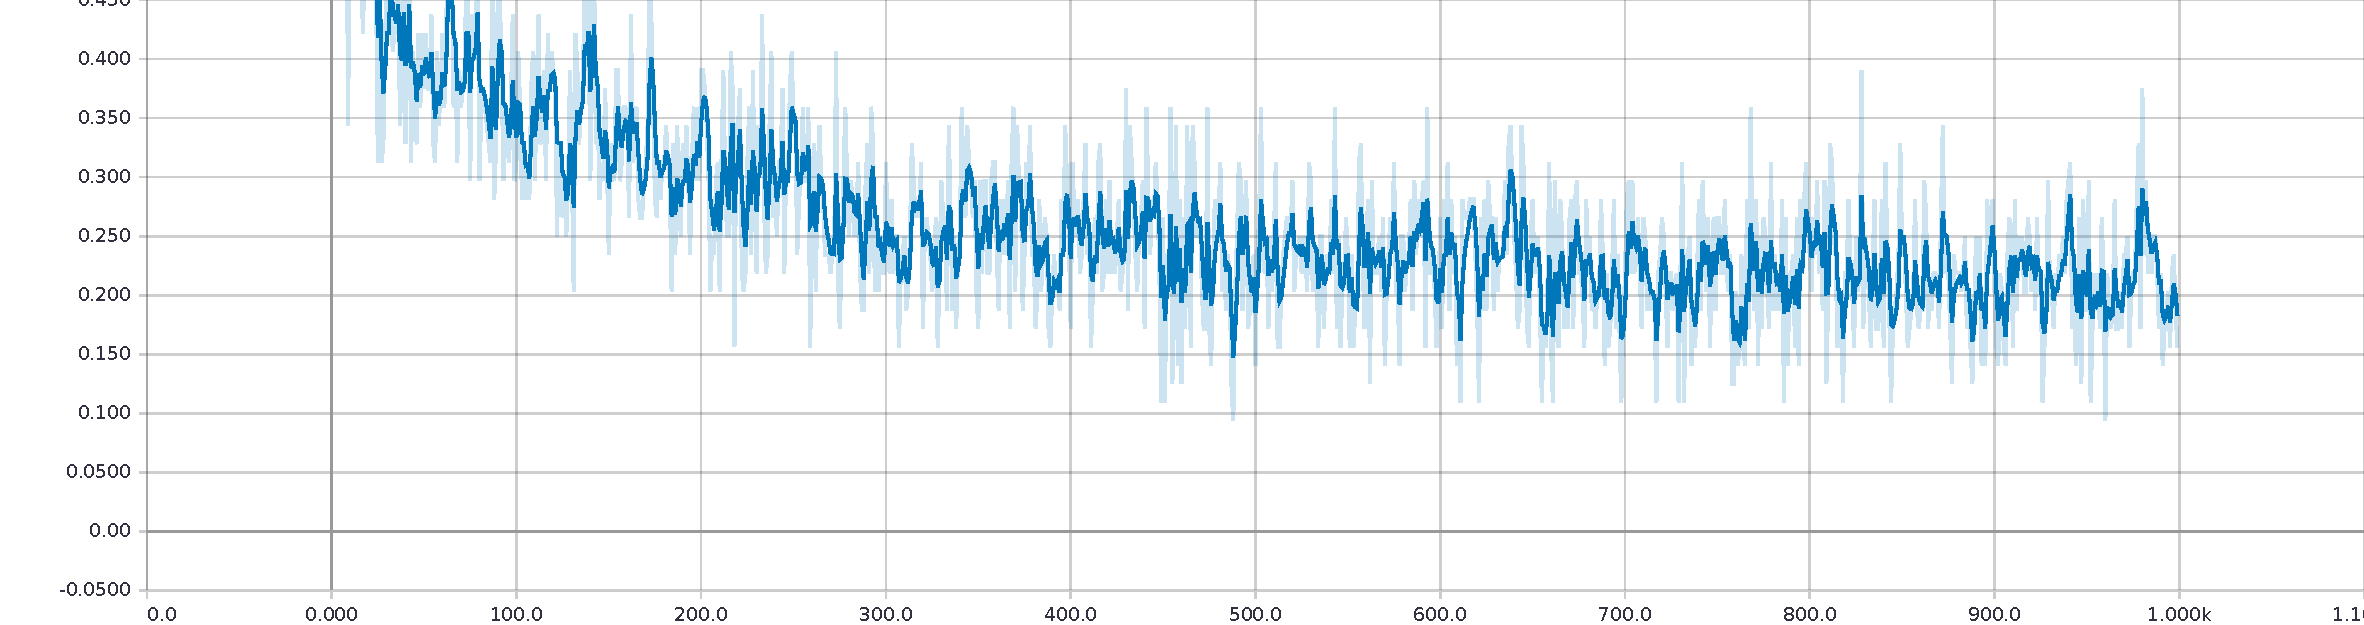
\includegraphics[width=16cm]{../images/improved_train_error.pdf}
    \caption{Error of the improved network during training}
    \label{Learning measurements}
  \end{center}
\end{figure}

\begin{figure}[H]
  \begin{center}
    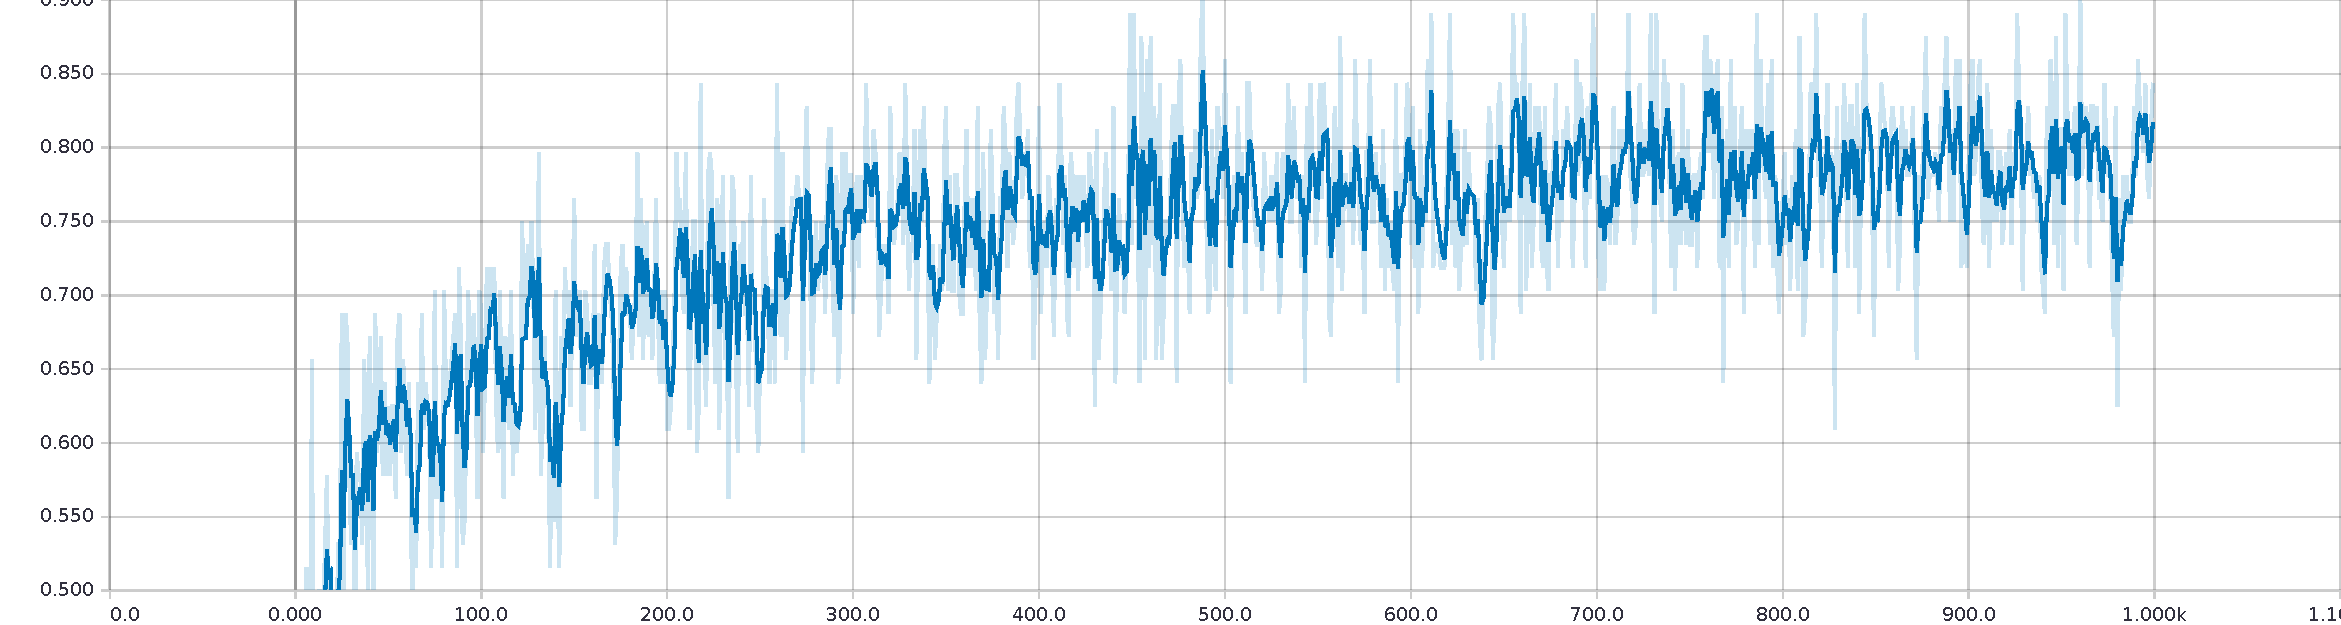
\includegraphics[width=16cm]{../images/improved_train_accuracy.pdf}
    \caption{Training accuracy of the improved network during training}
    \label{Learning measurements}
  \end{center}
\end{figure}

\begin{figure}[H]
  \begin{center}
    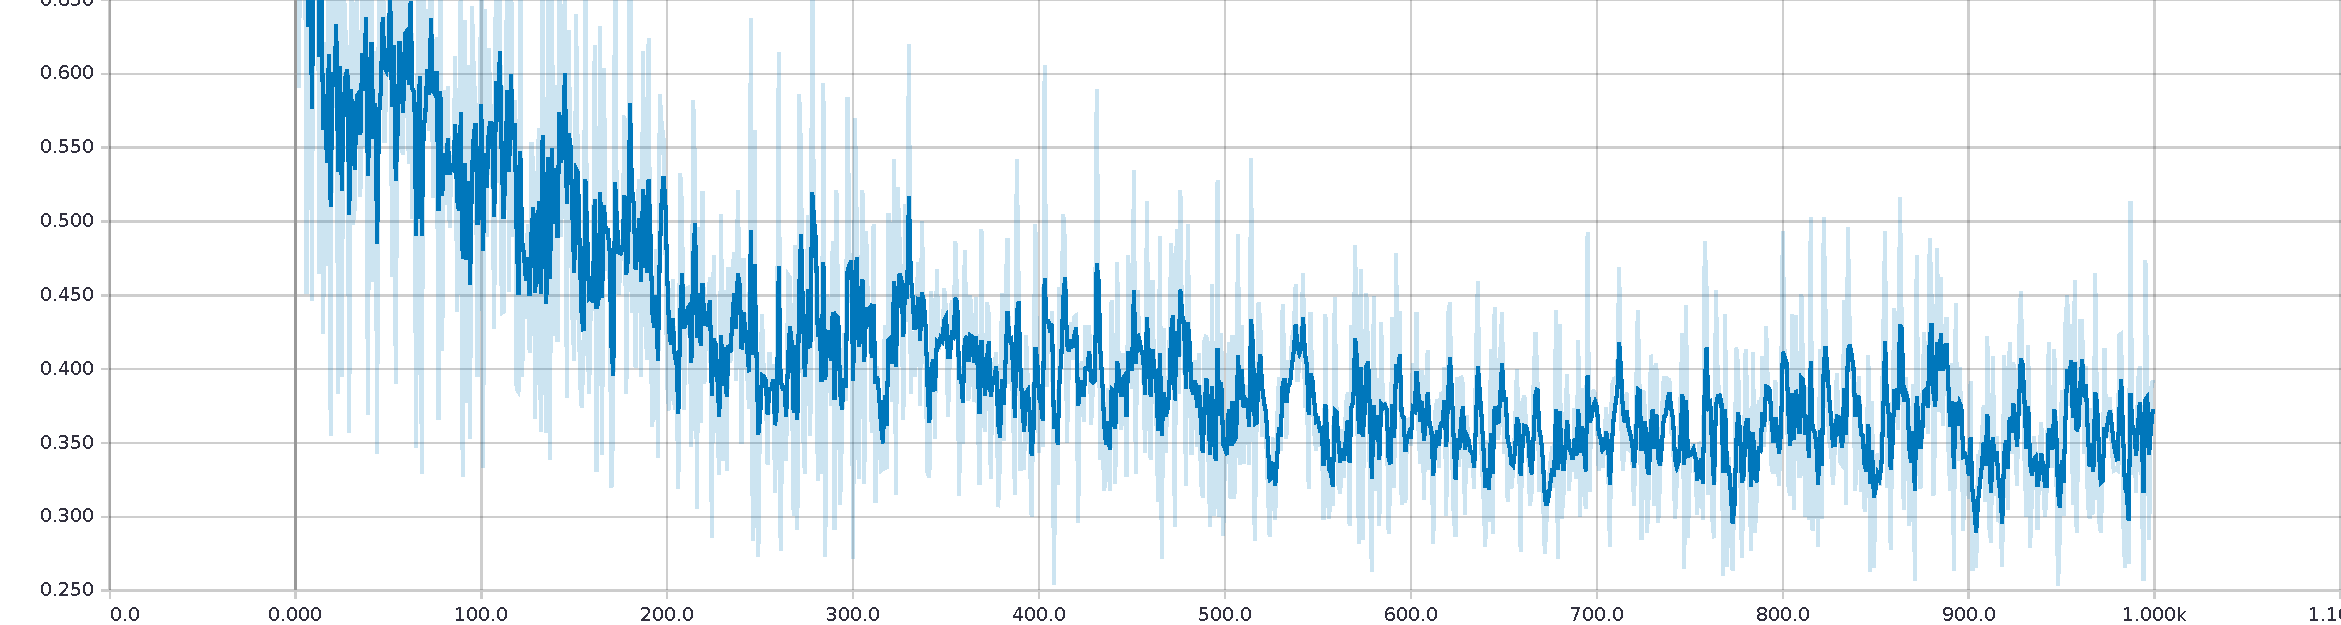
\includegraphics[width=16cm]{../images/improved_valid_error.pdf}
    \caption{Validation error of the improved network during training}
    \label{Learning measurements}
  \end{center}
\end{figure}

\begin{figure}[H]
  \begin{center}
    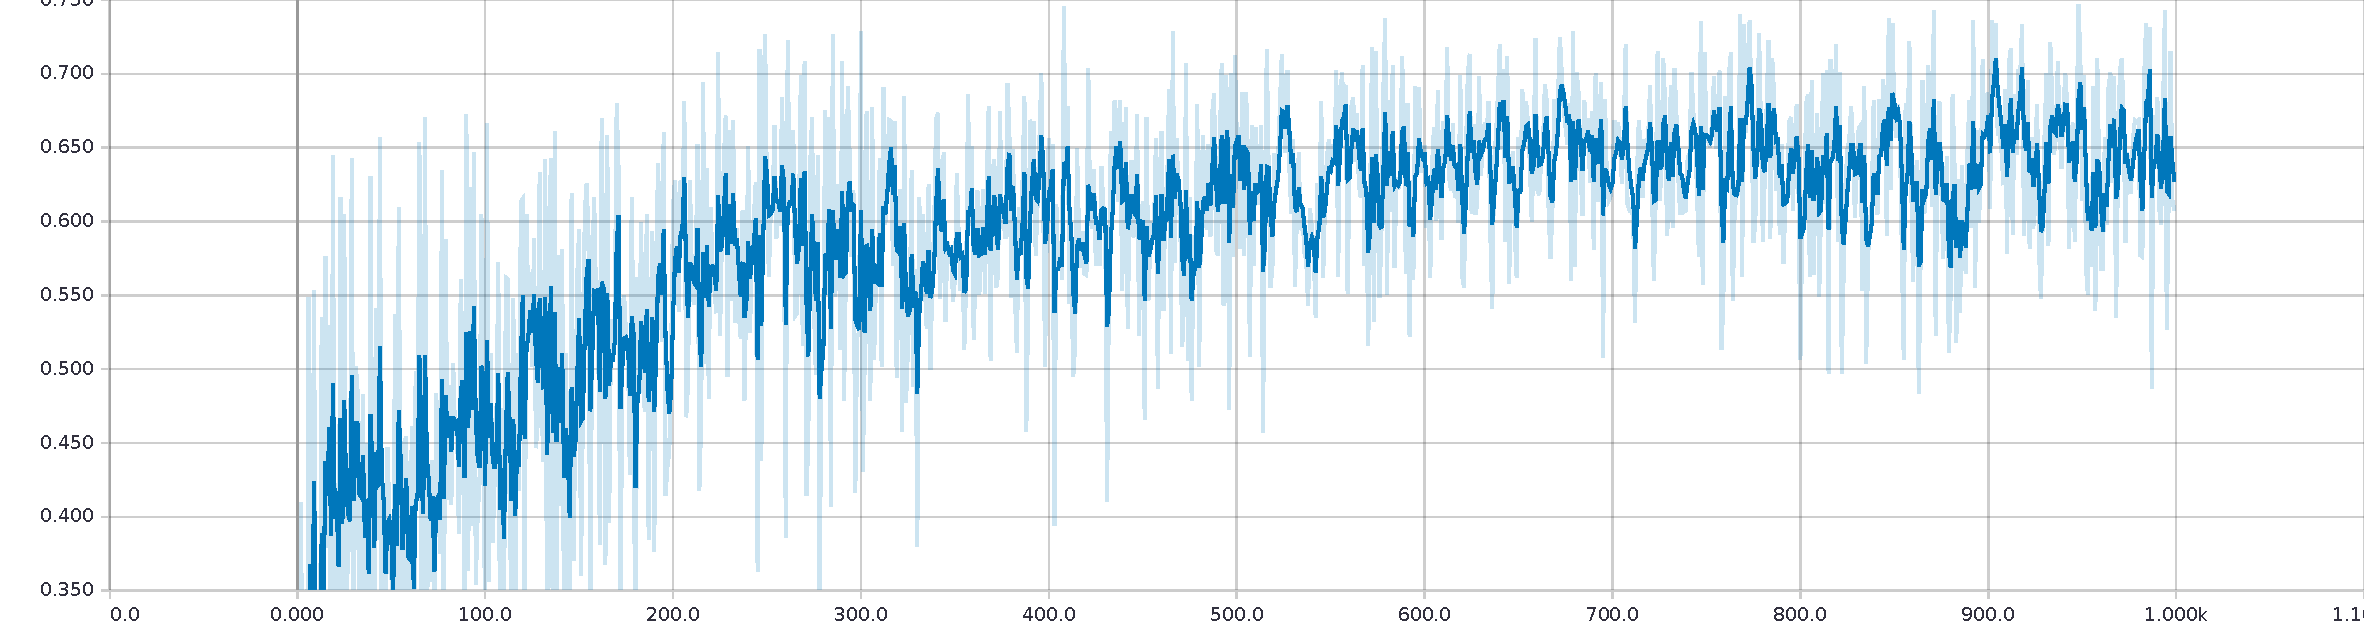
\includegraphics[width=16cm]{../images/improved_valid_accuracy.pdf}
    \caption{Validation accuracy of the improved network during training}
    \label{Learning measurements}
  \end{center}
\end{figure}

\begin{figure}[H]
  \begin{center}
    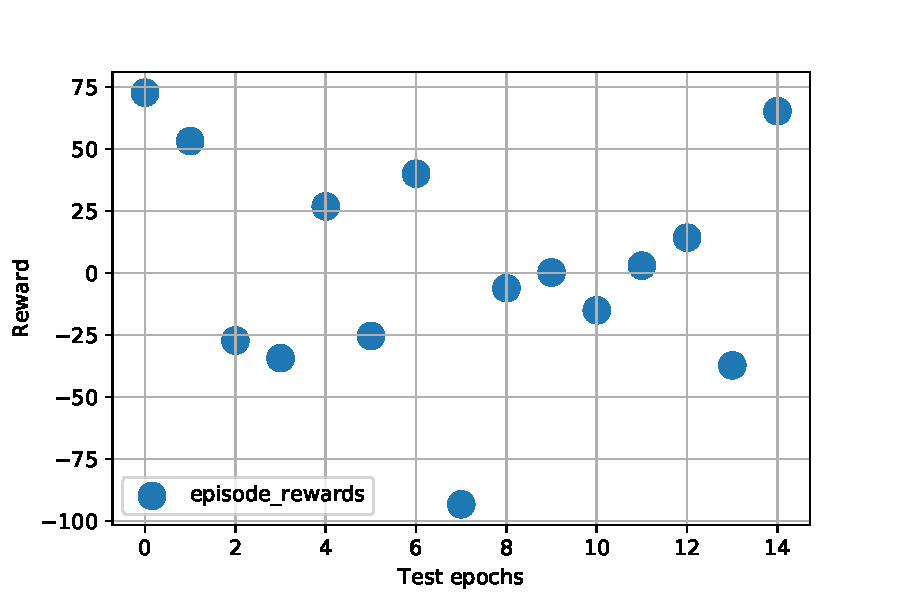
\includegraphics[width=16cm]{../images/Reward_of_Agent.pdf}
    \caption{Rewards of the improved agent in the test run}
    \label{Learning measurements}
  \end{center}
\end{figure}

\section{Influence of hyperparameters}
The longer the network trained, the better the results were. It took very long
to train the models on my laptop so I did not manage to run many hyper parameter
settings.

The networks performance depended on the expert's score somewhat but as it did
not manage to closely follow the expert's driving behavior anyway, it did not
change to much in our case.

And I did not manage to add the history working properly, due to my wedding last
friday.

But I guess, adding some kind of time dependency could improve the agent very much.
Standing still would rarely happen in the expert data und therefore should be penalized
in training.

\end{document}
